
\documentclass[tikz]{standalone}

\usepackage{tikz}


\begin{document}
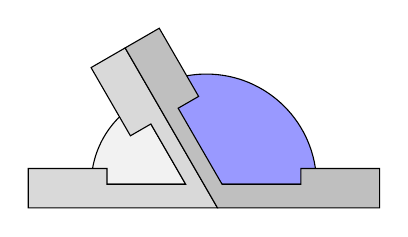
\begin{tikzpicture}


\def\l{1}
\def\d{.2}
\def\h{.3}

\def\angle{60}


\pgfmathsetmacro{\xx}{\h/tan(\angle)}
\pgfmathsetmacro{\xxx}{\d/sin(\angle)}

\draw[fill=gray!10] (-\xxx,0) --++(180:1.2)arc(180:180-\angle:1.2)--cycle;
\draw[fill=blue!40] (\xxx, 0) --++(0:1.2)arc(0:180-\angle:1.4)--cycle;


\pgfmathsetmacro{\x}{\l-\d/tan(\angle)}
\draw[fill=gray!30] (0,0) --++(180-\angle:\l+1)--++(270-\angle:.5)--++(-\angle:1)--++(90-\angle:.5-\d)--++(-\angle:\x)coordinate(1)--++(-1,0)--++(0,.2)--++(-1,0)|-(\xx,-\h)--cycle;

\pgfmathsetmacro{\x}{\l+\d/tan(\angle)}
\draw[fill=gray!50] (0,0) --++(180-\angle:\l+1)--++(90-\angle:.5)--++(-\angle:1)--++(-90-\angle:.5-\d)--++(-\angle:\x)coordinate(2)--++(1,0)--++(0,.2)--++(1,0)|-(\xx,-\h)--cycle;




\end{tikzpicture}
\end{document}